
% To do: Check optimilaity claims

\documentclass[10pt, conference, letterpaper]{IEEEtran}



%
% If IEEEtran.cls has not been installed into the LaTeX system files,
% manually specify the path to it like:
% \documentclass[10pt,journal,compsoc]{../sty/IEEEtran}


% Some very useful LaTeX packages include:
% (uncomment the ones you want to load)


% *** MISC UTILITY PACKAGES ***
%
%\usepackage{ifpdf}
% Heiko Oberdiek's ifpdf.sty is very useful if you need conditional
% compilation based on whether the output is pdf or dvi.
% usage:
% \ifpdf
%   % pdf code
% \else
%   % dvi code
% \fi
% The latest version of ifpdf.sty can be obtained from:
% http://www.ctan.org/tex-archive/macros/latex/contrib/oberdiek/
% Also, note that IEEEtran.cls V1.7 and later provides a builtin
% \ifCLASSINFOpdf conditional that works the same way.
% When switching from latex to pdflatex and vice-versa, the compiler may
% have to be run twice to clear warning/error messages.

\usepackage{upgreek}
% *** CITATION PACKAGES ***
%
\ifCLASSOPTIONcompsoc
  % IEEE Computer Society needs nocompress option
  % requires cite.sty v4.0 or later (November 2003)
  \usepackage[nocompress]{cite}
\else
  % normal IEEE
  \usepackage{cite}
\fi


% cite.sty was written by Donald Arseneau
% V1.6 and later of IEEEtran pre-defines the format of the cite.sty package
% \cite{} output to follow that of IEEE. Loading the cite package will
% result in citation numbers being automatically sorted and properly
% "compressed/ranged". e.g., [1], [9], [2], [7], [5], [6] without using
% cite.sty will become [1], [2], [5]--[7], [9] using cite.sty. cite.sty's
% \cite will automatically add leading space, if needed. Use cite.sty's
% noadjust option (cite.sty V3.8 and later) if you want to turn this off
% such as if a citation ever needs to be enclosed in parenthesis.
% cite.sty is already installed on most LaTeX systems. Be sure and use
% version 5.0 (2009-03-20) and later if using hyperref.sty.
% The latest version can be obtained at:
% http://www.ctan.org/tex-archive/macros/latex/contrib/cite/
% The documentation is contained in the cite.sty file itself.
%
% Note that some packages require special options to format as the Computer
% Society requires. In particular, Computer Society  papers do not use
% compressed citation ranges as is done in typical IEEE papers
% (e.g., [1]-[4]). Instead, they list every citation separately in order
% (e.g., [1], [2], [3], [4]). To get the latter we need to load the cite
% package with the nocompress option which is supported by cite.sty v4.0
% and later. Note also the use of a CLASSOPTION conditional provided by
% IEEEtran.cls V1.7 and later.
% *** GRAPHICS RELATED PACKAGES ***
%
\ifCLASSINFOpdf
   \usepackage[pdftex]{graphicx}
   \usepackage{subfigure}
  % declare the path(s) where your graphic files are
  % \graphicspath{{../pdf/}{../jpeg/}}
  % and their extensions so you won't have to specify these with
  % every instance of \includegraphics
  % \DeclareGraphicsExtensions{.pdf,.jpeg,.png}
\else
  % or other class option (dvipsone, dvipdf, if not using dvips). graphicx
  % will default to the driver specified in the system graphics.cfg if no
  % driver is specified.
   \usepackage[dvips]{graphicx}
   \usepackage{subfigure}
  % declare the path(s) where your graphic files are
  % \graphicspath{{../eps/}}
  % and their extensions so you won't have to specify these with
  % every instance of \includegraphics
  % \DeclareGraphicsExtensions{.eps}
\fi


% graphicx was written by David Carlisle and Sebastian Rahtz. It is
% required if you want graphics, photos, etc. graphicx.sty is already
% installed on most LaTeX systems. The latest version and documentation
% can be obtained at: 
% http://www.ctan.org/tex-archive/macros/latex/required/graphics/
% Another good source of documentation is "Using Imported Graphics in
% LaTeX2e" by Keith Reckdahl which can be found at:
% http://www.ctan.org/tex-archive/info/epslatex/
%
% latex, and pdflatex in dvi mode, support graphics in encapsulated
% postscript (.eps) format. pdflatex in pdf mode supports graphics
% in .pdf, .jpeg, .png and .mps (metapost) formats. Users should ensure
% that all non-photo figures use a vector format (.eps, .pdf, .mps) and
% not a bitmapped formats (.jpeg, .png). IEEE frowns on bitmapped formats
% which can result in "jaggedy"/blurry rendering of lines and letters as
% well as large increases in file sizes.
%
% You can find documentation about the pdfTeX application at:
% http://www.tug.org/applications/pdftex
% *** MATH PACKAGES ***
%
\usepackage[cmex10]{amsmath}
\usepackage{amssymb}
 \usepackage{graphicx}
 \usepackage{epstopdf}
  \usepackage{tabulary}
  \usepackage{array,booktabs,longtable,tabularx}
% A popular package from the American Mathematical Society that provides
% many useful and powerful commands for dealing with mathematics. If using
% it, be sure to load this package with the cmex10 option to ensure that
% only type 1 fonts will utilized at all point sizes. Without this option,
% it is possible that some math symbols, particularly those within
% footnotes, will be rendered in bitmap form which will result in a
% document that cannot be IEEE Xplore compliant!
%
% Also, note that the amsmath package sets \interdisplaylinepenalty to 10000
% thus preventing page breaks from occurring within multiline equations. Use:
%\interdisplaylinepenalty=2500
% after loading amsmath to restore such page breaks as IEEEtran.cls normally
% does. amsmath.sty is already installed on most LaTeX systems. The latest
% version and documentation can be obtained at:
% http://www.ctan.org/tex-archive/macros/latex/required/amslatex/math/
% *** SPECIALIZED LIST PACKAGES ***
%
\usepackage[justification=centering]{caption}
\usepackage{url}
\usepackage{amsmath}
\usepackage{amsfonts}
\newtheorem{definition}{\noindent{\bf Definition}}
\newtheorem{lemma}{\noindent{\bf Lemma}}
\newtheorem{theorem}{\noindent{\bf Theorem}}
\newtheorem{proposition}{\noindent{\bf proposition}}



\usepackage{algorithm}
\usepackage{algorithmic}
% algorithmic.sty was written 

\usepackage{eqparbox}

\renewcommand{\algorithmiccomment}[1]{\hfill\eqparbox{COMMENT}{\%~#1}}




\begin{document}

\title{Yosemite: Efficient Scheduling of Weighted Coflows in Data Centers}
\author{\IEEEauthorblockN{Han Zhang\IEEEauthorrefmark{1}\IEEEauthorrefmark{3},  Xingang Shi\IEEEauthorrefmark{2}\IEEEauthorrefmark{3}, Xia Yin\IEEEauthorrefmark{1}\IEEEauthorrefmark{3}, Zhiliang Wang\IEEEauthorrefmark{2}\IEEEauthorrefmark{3}}
\IEEEauthorblockA{\IEEEauthorrefmark{1}Department of Computer Science and Technology, Tsinghua University\\
\IEEEauthorrefmark{2}Institute for Network Sciences and Cyberspace, Tsinghua University\\
\IEEEauthorrefmark{3}Tsinghua National Laboratory for Information Science and Technology (TNLIST)\\
Beijing, P.R. China\\
Email:\{zhanghan, wzl, yxia\}@csnet1.cs.tsinghua.edu.cn, \{shixg\}@cernet.edu.cn
}
}
% make the title area
\maketitle



\begin{abstract}
Recently, coflow has been proposed as a new abstraction to capture the communication patterns in a rich set of data parallel applications in data centers. Coflows effectively model the application-level semantics of network resource usage, so high-level optimization goals, such as reducing the transfer latency of applications, can be better achieved by taking coflows as the basic elements in network resource allocation or scheduling.
Although efficient coflow scheduling methods have been studied, in this paper, we propose to schedule {\em weighted coflows} as a further step in this direction, where weights are used to express the emergences or priorities of different coflows or their corresponding applications. We design an information-agnostic online algorithm to dynamically schedule coflows according to their weights and the instantaneous network condition. Then We implement the algorithm in a scheduling system named Yosemite. Our evaluation results show that, compared to the latest information-agnostic coflow scheduling algorithms, Yosemite can reduce more than 40\% of the WCCT (Weighted Coflow Completion Time) , and more than 30\% of the completion time for coflows with above-the-average level of emergence. It even outperforms the most efficient clairvoyant coflow scheduling method by reducing around 30\% WCCT, and 25\%$\sim$30\% of the completion time for coflows with above-the-average emergence, respectively. %Nowadays, applications (hadoop, ceph, etc.) in data center need network to provide them with low latency and high throughput. 
%However, as resources of data center network are limited, efficient network schedule methods are needed. Recently, the proposed
%application level abstraction coflow tries to regard flows of data-parallel applications as a whole, so that transfer latency of applications will be reduced. 
%For reducing application transfer latency, application level optimization methods perform better than flow level ones.
%This is because often a application's communication stage cannot finish until all its flows have completed. 
%Although coflow level scheduling methods such as Varys and Aalo perform well on reducing application transfer latency,
%they ignore different applications always have different level of emergence and 
%scheduling just depends on network condition and characters (width, length) of coflows is not enough.
%In reality, the emergence of applications should also be taken into consideration.
%In this paper, we incorporate weight to present the emergence of applications and try to minimize average coflow weight completion time.
%To achieve this, we design Yosemite-a system that aims to minimize average weight coflow completion time.
%We test Yosemite's performance in trace-driven simulation as well as our cloud platform and then compare its performance with state-of-art methods.  
%Trace-driven simulation shows that Yosemite performs about 20\%$\sim$50\%better than Varys and 30\%$\sim$60\% better than Aalo. 
%Testbed evaluation shows Yosemite performs  30\% and 35\% better than Varys and Aalo respectively on average.
\end{abstract}

\section{Introduction}\label{introduction}

Recently, coflow has been proposed as a new abstraction to capture the communication patterns in a rich set of data parallel applications.
According to \cite{chowdhury2014efficient}, a coflow is {\em a collection of flows between two groups of machines with associated semantics and a collective objective.} The collection of flows share a common performance goal, e.g., minimizing the completion time of the latest flow in the collection, or ensuring that flows in the collection meet a common deadline. 
Coflows effectively model the application-level semantics of network resource usage, so high-level optimization goals, such as reducing the transfer latency of applications, can be better achieved by taking coflows as the basic elements in network resource allocation or scheduling.
Efficient coflow scheduling methods targeting minimizing Coflow Completion Time (CCT) have been studied. 
Varys \cite{chowdhury2014efficient} proposes the {\em Smallest-Effective-Bottleneck-First} (SEBF) heuristic to determine the scheduling order of coflows and uses {\em Minimum-Allocation-for-Desired-Duration} (MADD) to compute the bandwidth to be allocated. However, Varys is a clairvoyant method in the sense that it depends on flow information, such as flow size or flow arrival time, to determine how to scheduling coflows. This may limit its application to scenarios where such information cannot be provided a priori. To solve this problem, non-clairvoyant methods that are flow information agnostic, such as Aalo \cite{chowdhury2015efficient}, Barrat \cite{dogar2014decentralized},and CODA \cite{zhang2016coda}, have also been studied.
In this paper, we propose to schedule {\em weighted coflows} as a further step in this direction, where weights are assigned to coflows to express the emergences or priorities of different coflows or their corresponding applications. We design an information-agnostic online algorithm to dynamically schedule coflows according to their weights and the instantaneous network condition. 

\section{Motivation} \label{motivation}

\begin{figure}[!t]
\centering
\subfigure[Average CCT] {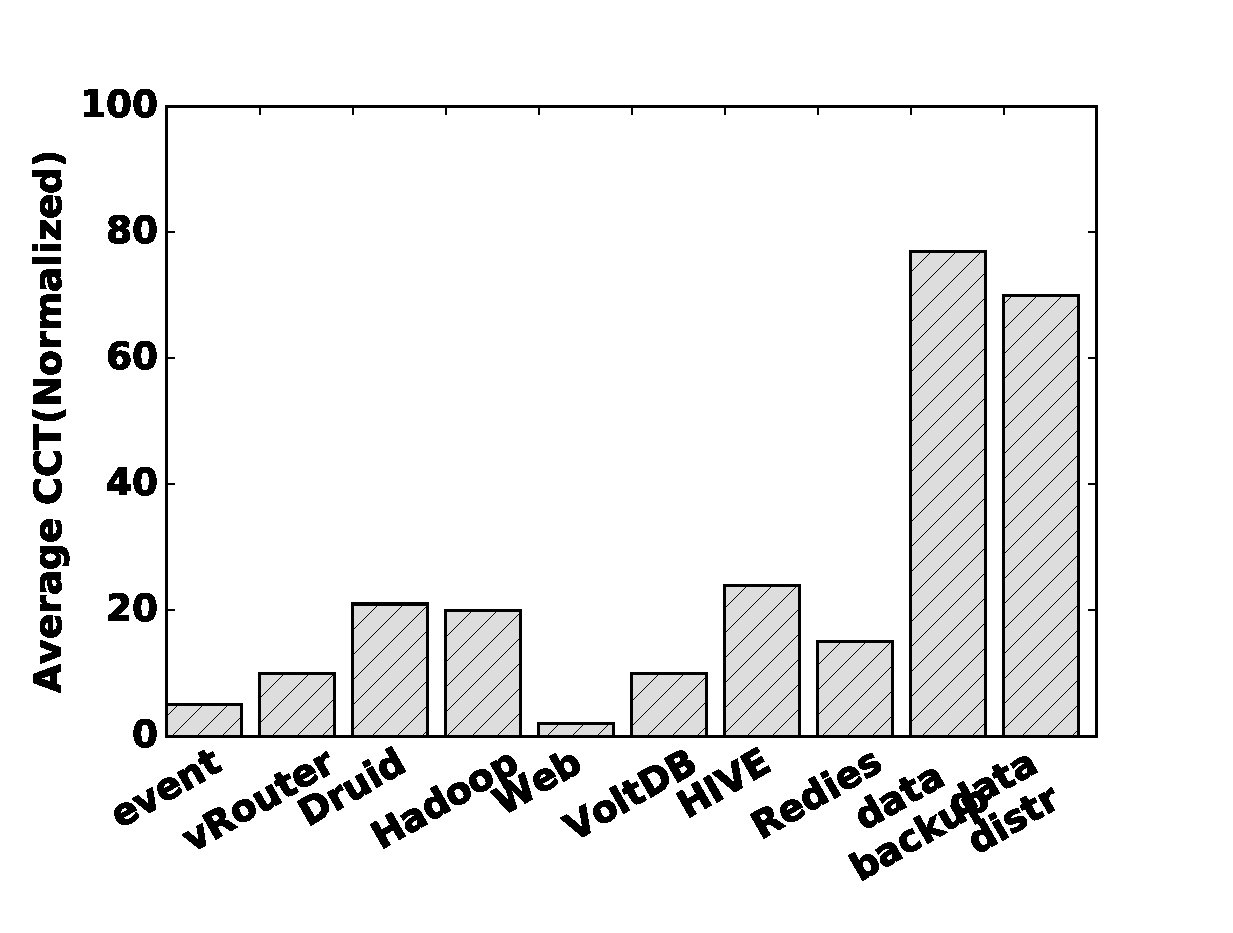
\includegraphics[width=1.5 in]{./figs/motivation/motivation1.eps}}
\hspace{0.1in}
\subfigure[Average CCT with Varys ] {\includegraphics[width=1.5 in]{./figs/motivation/motivation3.eps}}
\hspace{0.1in}
\caption{Normalized Coflow Completion Time, grouped by the level of emergence}
\label{motivation_fig}
\vspace{-0.1 in}
\end{figure}

We now use real network traffic from a medium-sized data center, where more than 100 applications run on about 3000 servers simultaneously. After talking with the network operators and software development engineers about the emergence of different applications, we make an in-depth analysis of the traffic collected from 720 servers deployed in 60 racks. The traffic lasts about one month, and the basic statistics of the top ten network-demanding applications are summarized in Table \ref{tab:measure}. There are typically five emergence levels, i.e., significant, important, normal, unimportant and lax. For example, the event application and the vRoute application are responsible for communication of critical components, and are of the highest level of emergence, while data-backup and data-dist are  applications running in the background and are of the lowest level of emergence. 
To illustrate the ineffectiveness of existing coflow scheduling methods, we plot the average Coflow Completion Time (CCT) of different coflows, grouped by their levels of emergence, in Fig.\ref{motivation_fig}. Fig.\ref{motivation_fig}(a) shows the direct measurement result of all applications, while Fig.\ref{motivation_fig}(b) shows the simulation result when Varys is used to schedule them. Comparing the two plots, we can see that Varys clearly reduces the completion time of less emergent coflows, such as Redies, data-backup and data-dist, at the expenses of the same of even longer completion time of more emergent coflows, such as Event and vRouter. This motivates us to optimize the Weighted Coflow Completion Time (WCCT), where weight denotes the emergence of coflows, and the more emergent the coflow, the higher the weight. Coflow scheduling algorithms should take coflow weight into consideration, and optimizing CCT becomes just a special case of optimizing WCCT.


 \begin{table}[!htb]
\centering
\footnotesize
 \caption{Applications and their levels of emergence} \label{tab:measure}
\begin{tabulary}{\textwidth}{rccccr}
\toprule
App Name  & \multicolumn{1}{c}{Type} &  width&  length (MB)&Emergence Level\\
\midrule
 \multicolumn{1}{r}{Event} &     communication    &20&5     &  significant \\
 \multicolumn{1}{r}{vRouter} &  communication     &8&3 &  significant\\
\multicolumn{1}{r}{Druid} &     interactive   &6&18   &  important \\
\multicolumn{1}{r}{Hadoop} &  computation  &5&42     &  normal \\
 \multicolumn{1}{r}{Web} &     interactive   &3&5     &  normal\\
\multicolumn{1}{r}{VoltDB} &     background  &4&21    &  normal\\
 \multicolumn{1}{r}{Hive} &     background   &7&32     &  unimportant \\
   \multicolumn{1}{r}{Redies} &    background   &2&30    &  unimportant \\
    \multicolumn{1}{r}{data-backup} &    background   &3&124     &  lax \\
     \multicolumn{1}{r}{data-dist} & background      &5&93  &lax \\
\bottomrule
 \end{tabulary}
 \end{table}

\section{Algorithm}
 \begin{algorithm} 
 \caption{Information-agnostic Online scheduling to minimize WCCT}
 \begin{algorithmic}[1]\label{online-algorithm}
% \renewcommand{\algorithmicrequire}{\textbf{Input: }}
% \renewcommand{\algorithmicensure}{\textbf{Output:}}
% \REQUIRE  Coflow $F^{(k)}$ ;  $s_{i,j}^{(k)}$ that has been sent from port i to port j for Coflow $F^{(k)}$, where $1 \leqslant i\leqslant m$,$1 \leqslant j \leqslant m$
% \ENSURE  $\gamma$
  \IF{a new coflow arrives}
  \STATE update the coflow list $\mathcal{F}=\{F^{(k)}\}$
  \STATE $n=|\mathcal{F}|$
  \FOR{$1 \le k \le n$ } 
    \STATE update $s_{i,j}^{(k)}$, the cumulative volume of the traffic sent by coflow $F^{(k)}$, for $1 \le i, j \le m$
    \STATE $L_i^{(k)}= \sum_{j=1}^ms_{i,j}^{(k)}$ for $1 \le i \le m$
    \STATE $L_{j+m}^{(k)}= \sum_{i=1}^ms_{i,j}^{(k)}$ for $1 \le j \le m$
    \STATE $l^{(k)}$=$ \min \limits_{1 \le i \le 2m}L_i^{(k)}$
    \STATE $\alpha^{(k)}=l^{(k)}/w_k$
  \ENDFOR
  \STATE $\omega=$sort the list of $\{\alpha^{(k)}\}$ in nondecreasing order
  \STATE $\gamma=$index set of $\omega$
  \ENDIF
  \STATE initialize the bandwidth to be allocated on each ingress and egress port: $I_p=O_p=$ port physical bandwidth, for $1 \le p \le m$
  \FOR{$\ell$ from 1 to $n$}
    \STATE schedule coflow $F=F^{(\gamma[\ell])}$
    \STATE $r$ = min $\{I_p, O_q\}$, subject to $F$ still need to send traffic to port $p$ or receive traffic from port $q$
    \FOR{each unfinished flow $F_{i,j}$ in $F$} 
      \STATE allocate bandwith of $r$ to $F_{i,j}$
      \STATE update $I_i$ and $O_j$ by deducting $r$ from them 
    \ENDFOR
  \ENDFOR
  \STATE allocate remaining bandwidth equally to all flows
 \end{algorithmic} 
 \end{algorithm}
 
 \begin{figure}[!t]
\centering
\subfigure[Average CCT] {\includegraphics[width=3 in]{./figs/evaluation/ex1/evaluation_motivation2.eps}}
\vspace{-0.1 in}
\caption{[Simulation] Average CCT (Normalized)  and Average WCCT for all applications}
\label{evaluation_motivation_fig}
\vspace{-0.1 in}
\end{figure}

Efficient algorithm is needed to schedule coflows according to the network condition and emergence level.
Algorithm \ref{online-algorithm} prioritizes coflows according to the heuristics explained above (line 1 $\sim$ 13) and allocates bandwidth to each flow (line 14 $\sim$ 22). At last, it distributes the unallocated bandwidth equally among all unfinished flows to provide resource conservation.
Algorithm \ref{online-algorithm}  is an information-agnostic online algorithm that dynamically schedule coflows according to their weights and the instantaneous network condition.


To test the performance of this.  We set 5 level of emergence in our data center and use 5, 4, 3 ,2, 1 to present the Significant, Important, Normal, Unimportant and Lax level of emergence, then Fig. \ref{evaluation_motivation_fig} shows the result.
%Fig. \ref{evaluation_motivation_fig}(a) shows average WCCT for all coflows.
%We can see the Normalized WCCT of Varys are 8 (Narrow\&Short), 20(Narrow\&Long), 15 (Wide\&Short), 40  (Wide\&Long) and 30(ALL),
%while that for Yosemite are  5 (Narrow\&Short), 15(Narrow\&Long), 10 (Wide\&Short), 30  (Wide\&Long) and 20(ALL).
%Yosemite performs about 20\% better than Varys on minimizing average WCCT.
%From Fig. \ref{evaluation_motivation_fig}(b) 
We can see that for vRouter and event which own significant level emergence,
Varys performs almost to TCP, while Yosemite performs about 20\% better than TCP.
For Hadoop and Druid (Important), Yosemite performs about 30\% better than Varys.
While other unimportant applications Varys perform about 10\%$\sim$20\% better than Yosemite.


\bibliographystyle{abbrv}
\bibliography{paper}



\end{document}



